\documentclass[tikz,border=6pt]{standalone}
\usetikzlibrary{arrows.meta,decorations.pathreplacing,calc}
\begin{document}
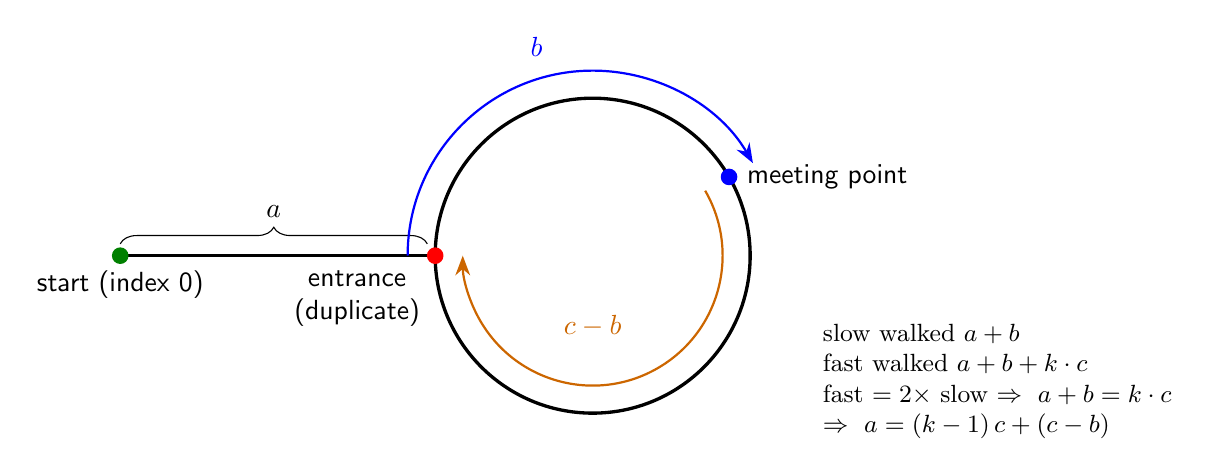
\begin{tikzpicture}[font=\sffamily,ar/.style={-{Stealth[length=2.5mm]},thick}]
\coordinate (S) at (0,0); \coordinate (E) at (4,0);
\draw[very thick] (S)--(E);
\draw[very thick] (6,0) circle (2);
\fill[green!50!black] (S) circle (3pt) node[below=2pt,black] {start (index 0)};
\fill[red] (E) circle (3pt) node[below left=2pt,black,align=center] {entrance\\(duplicate)};
\coordinate (M) at ($(6,0)+(30:2)$);
\fill[blue] (M) circle (3pt) node[right=3pt,black] {meeting point};
\draw[decorate,decoration={brace,amplitude=6pt}] (0,0.15)--(3.9,0.15) node[midway,above=6pt] {$a$};
\draw[ar,blue] ($(6,0)+(180:2.35)$) arc (180:30:2.35);
\node[blue] at ($(6,0)+(105:2.75)$) {$b$};
\draw[ar,orange!80!black] ($(6,0)+(30:1.65)$) arc (30:-180:1.65);
\node[orange!80!black] at (6,-0.9) {$c-b$};
\node[align=left,anchor=west,font=\small] at (8.8,-1.6) {slow walked $a+b$\\fast walked $a+b+k\cdot c$\\fast $=2\times$ slow $\Rightarrow\ a+b = k\cdot c$\\$\Rightarrow\ a = (k-1)\,c + (c-b)$};
\end{tikzpicture}
\end{document}
